\documentclass[a4paper,12pt,ngerman]{scrartcl}
\usepackage{babel}
\usepackage[T1]{fontenc}
\usepackage[utf8x]{inputenc}
\usepackage[a4paper,margin=2.5cm,footskip=0.5cm]{geometry}
% Die nächsten vier Felder bitte anpassen:
\newcommand{\Aufgabe}{OOP-Projekt: Kartennavigation}
\newcommand{\Namen}{JR}           % Namen der Bearbeiter/-innen dieser Aufgabe angeben
 
% Kopf- und Fußzeilen
\usepackage{scrlayer-scrpage, lastpage}
\setkomafont{pageheadfoot}{\large\textrm}
\lohead{\Aufgabe}
\cfoot*{\thepage{}/\pageref{LastPage}}

% Position des Titels
\usepackage{titling}
\setlength{\droptitle}{-1.0cm}

% Für mathematische Befehle und Symbole
\usepackage{amsmath}
\usepackage{amssymb}

% Für Bilder
\usepackage{graphicx}
\usepackage{wrapfig}

% Für Algorithmen
\usepackage{algpseudocode}

% Für Quelltext
\usepackage{listings}
\usepackage{color}
\definecolor{mygreen}{rgb}{0,0.6,0}
\definecolor{mygray}{rgb}{0.5,0.5,0.5}
\definecolor{mymauve}{rgb}{0.58,0,0.82}
\lstset{
  keywordstyle=\color{blue},commentstyle=\color{mygreen},
  stringstyle=\color{mymauve},rulecolor=\color{black},
  basicstyle=\footnotesize\ttfamily,numberstyle=\tiny\color{mygray},
  captionpos=b, % sets the caption-position to bottom
  keepspaces=true, % keeps spaces in text
  numbers=left, numbersep=5pt, showspaces=false,showstringspaces=true,
  showtabs=false, stepnumber=2, tabsize=2, title=\lstname,
  showstringspaces=false,
  literate={ö}{{\"o}}1 {ä}{{\"a}}1 {ü}{{\"u}}1 {ß}{{\ss}}1
}
\lstset{
extendedchars=\true,
inputencoding=utf8x
}
\lstdefinelanguage{JavaScript}{ % JavaScript ist als einzige Sprache noch nicht vordefiniert
  keywords={break, case, catch, continue, debugger, default, delete, do, else, finally, for, function, if, in, instanceof, new, return, switch, this, throw, try, typeof, var, void, while, with},
  morecomment=[l]{//},
  morecomment=[s]{/*}{*/},
  morestring=[b]',
  morestring=[b]",
  sensitive=true
}

% Diese beiden Pakete müssen zuletzt geladen werden
%\usepackage{hyperref} % Anklickbare Links im Dokument
\usepackage{hyperref}
\usepackage{cleveref}

\graphicspath{{./Bilder/}}

% Daten für die Titelseite
\title{\textbf{\Huge\Aufgabe}}
\author{\LARGE \Namen\\\\}
\date{\LARGE11. März 2024}
\begin{document}

\maketitle
\tableofcontents

\vspace{1cm}

Projekt verfügbar unter \url{https://kartennavigation.streamlit.app}

Code verfügbar unter \url{https://github.com/Jo-na-tan/Info_Projekt}

\section{Problemstellung und Kundenanforderungen}
Ziel des Projektes ist es, eine Karte von New York zu erstellen, die den kürzesten Weg zwischen zwei wählbaren Punkten anzeigt. Dabei soll der Kunde eine interaktive Karte erhalten, das heißt, sie kann bewegt werden und es kann hinein- und herausgezoomt werden. Auf dieser Karte soll es möglich sein, zwei Punkte zu wählen, zwischen denen sowohl die Route mit dem kürzesten Weg, als auch die Route mit der geringsten Zeit angezeigt wird. Weiterhin soll die kürzeste Zeit in Minuten und der kürzeste Weg in Meilen angegeben werden. Wenn ein Punkt gewählt wird, der nicht im Straßennetz vorhanden ist, soll der nächste Punkt des Straßennetzes als Start- beziehungsweise Endpunkt der Route benutzt werden. Dies soll mithilfe einer Webseite dargestellt werden, die dem Kunden jederzeit zur Verfügung steht. Auch soll diese Seite intuitiv und einfach zu bedienen sein.

\newpage
\section{Planung}
\begin{figure}[!ht]
  \center
  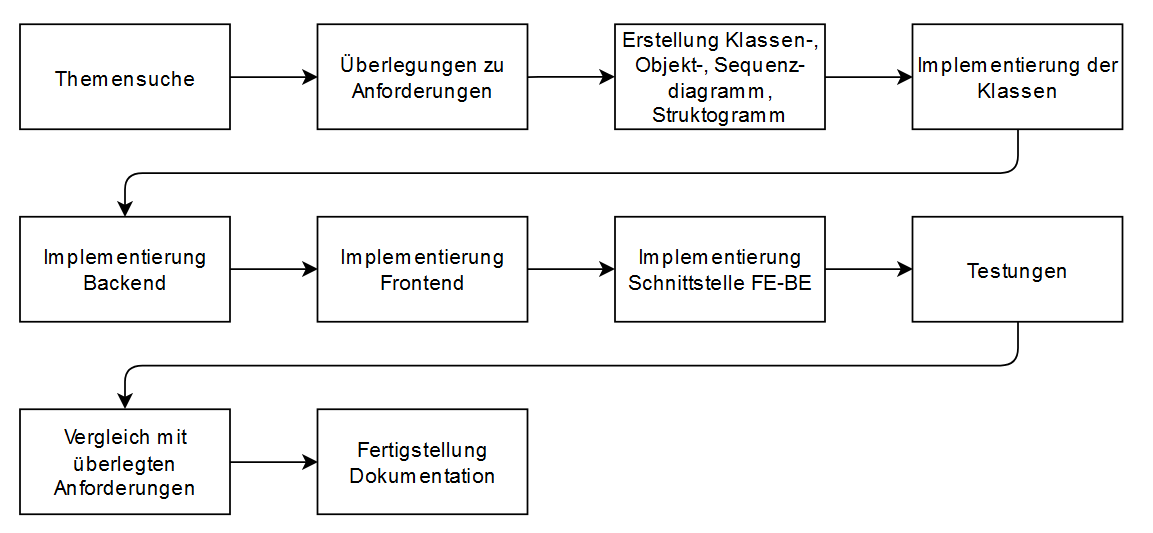
\includegraphics[width=\textwidth]{Pipelinediagramm.png}
  \vspace{-.5cm}
  \caption{Pipelinediagramm}
\end{figure}

\section{Analyse informatischer Anforderungen}
Um die Anforderungen zu erfüllen, wird bei der Routensuche mit objektorientierter Programmierung gearbeitet. Dabei sind Kanten, Knoten und Graphen Objekte mit den im Klassendiagramm dargestellten Attributen. Zunächst muss das Straßennetz mit txt-Dateien von \url{http://www.diag.uniroma1.it/challenge9/download.shtml} eingelesen (Kanten haben in den Dateien Zeit- und Wegangaben und Knoten haben Koordinaten) und in die Objekte überführt werden. Zum Berechnen der Routen für die geringste Zeit und kürzesten Weg wird der Dijkstra-Algorithmus mit Priority-Queue verwendet, der abbricht, wenn das Ziel gefunden wurde. Dafür muss allerdings zuerst der zum gewählten Startpunkt nächste Knoten des Straßennetzes gefunden werden, wobei alle Knoten durchgegangen werden und der mit dem kürzesten Abstand, der mit der Haversine-Formel berechnet wird, gewählt wird. Mit dem Paket folium können die Punkte und die Routen auf einer Karte angezeigt werden. Auch die Wahl von zwei Punkten wird mit diesem Paket ermöglicht. Mit streamlit und streamlit-folium kann ein Web-Interface erstellt werden, das mit der Routenberechnung verknüpft wird.

\newpage
\section{Diagramme}
\begin{figure}[!ht]
  \center
  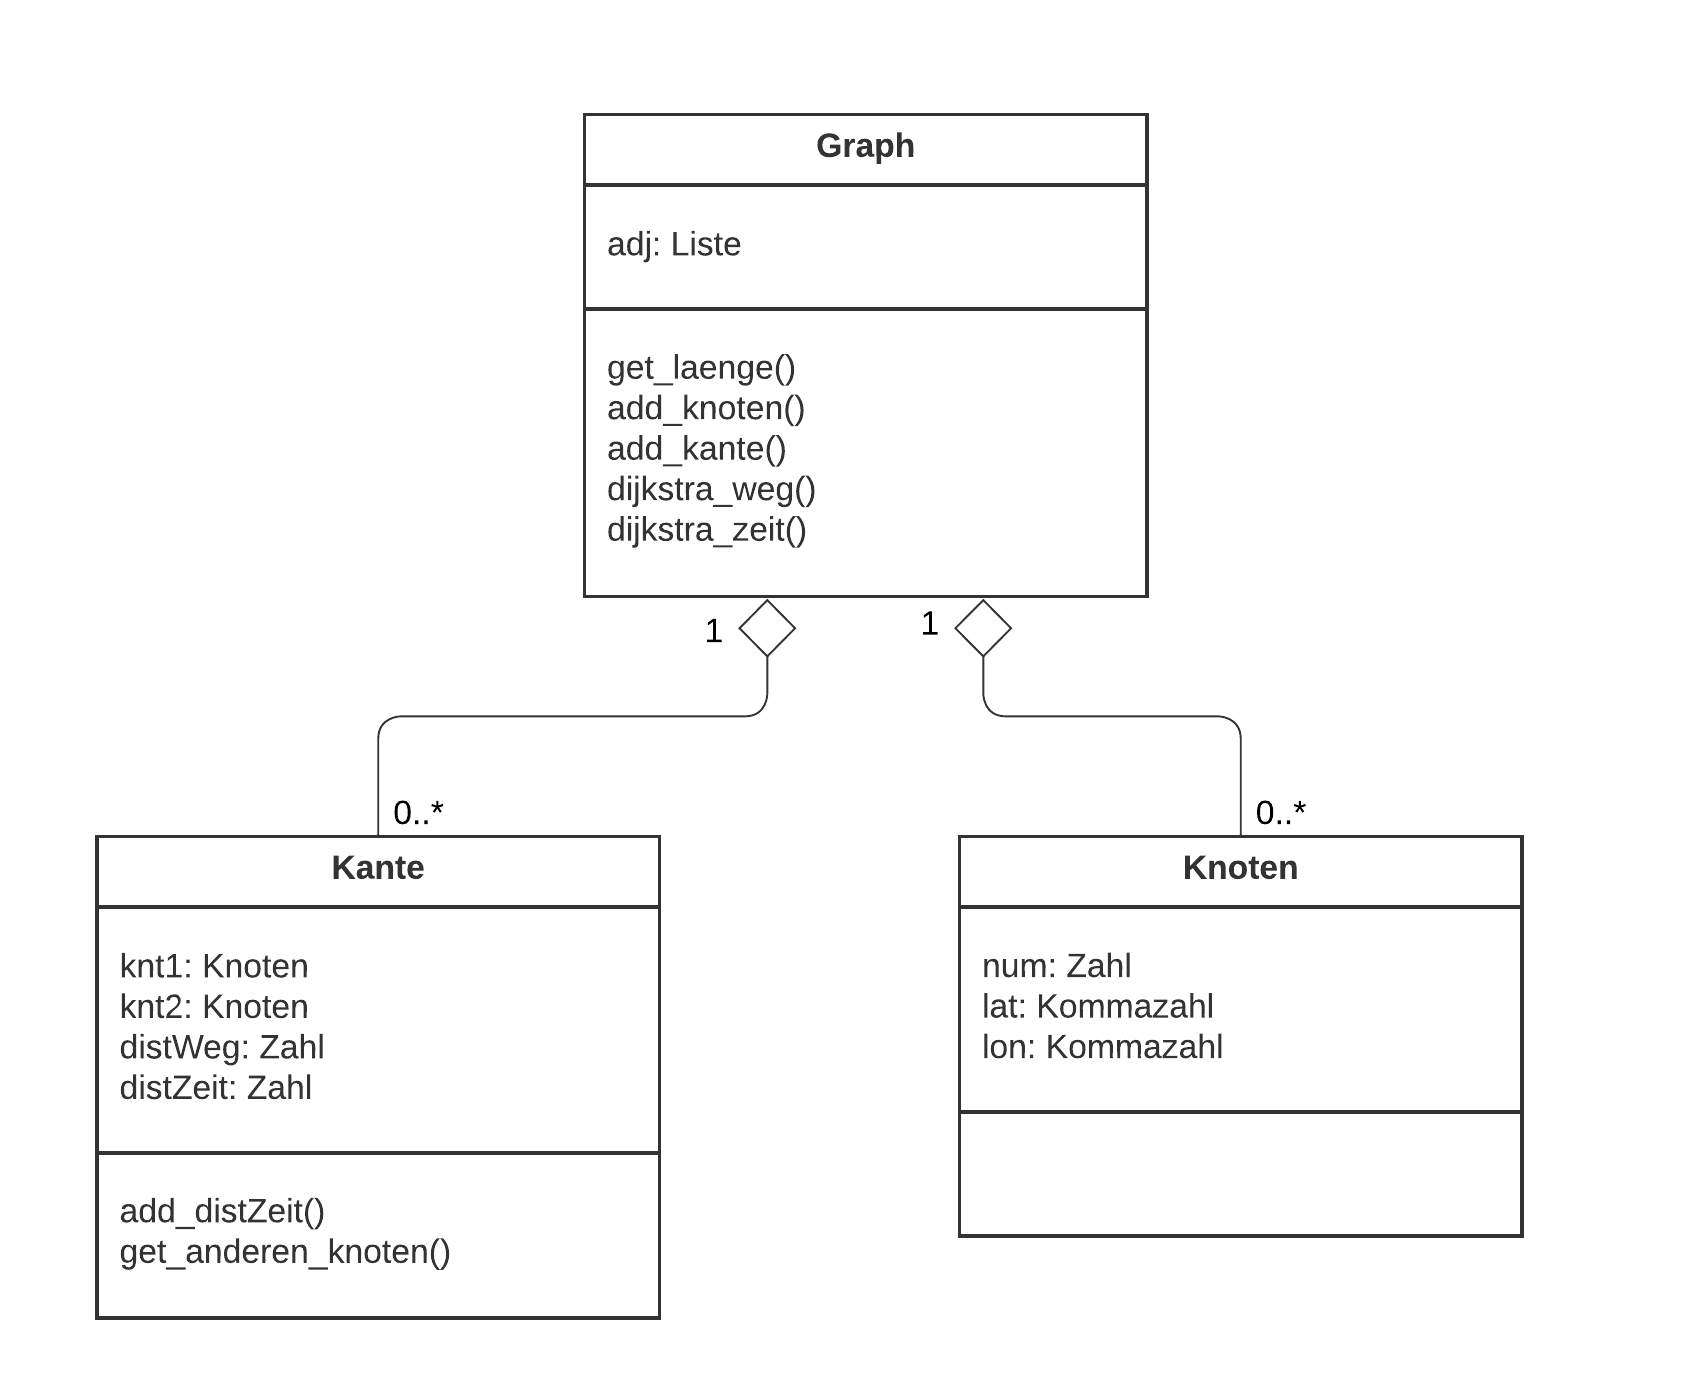
\includegraphics[width=\textwidth]{Klassendiagramm.png}
  \vspace{-.5cm}
  \caption{Klassendiagramm}
\end{figure}

\begin{figure}[!ht]
  \center
  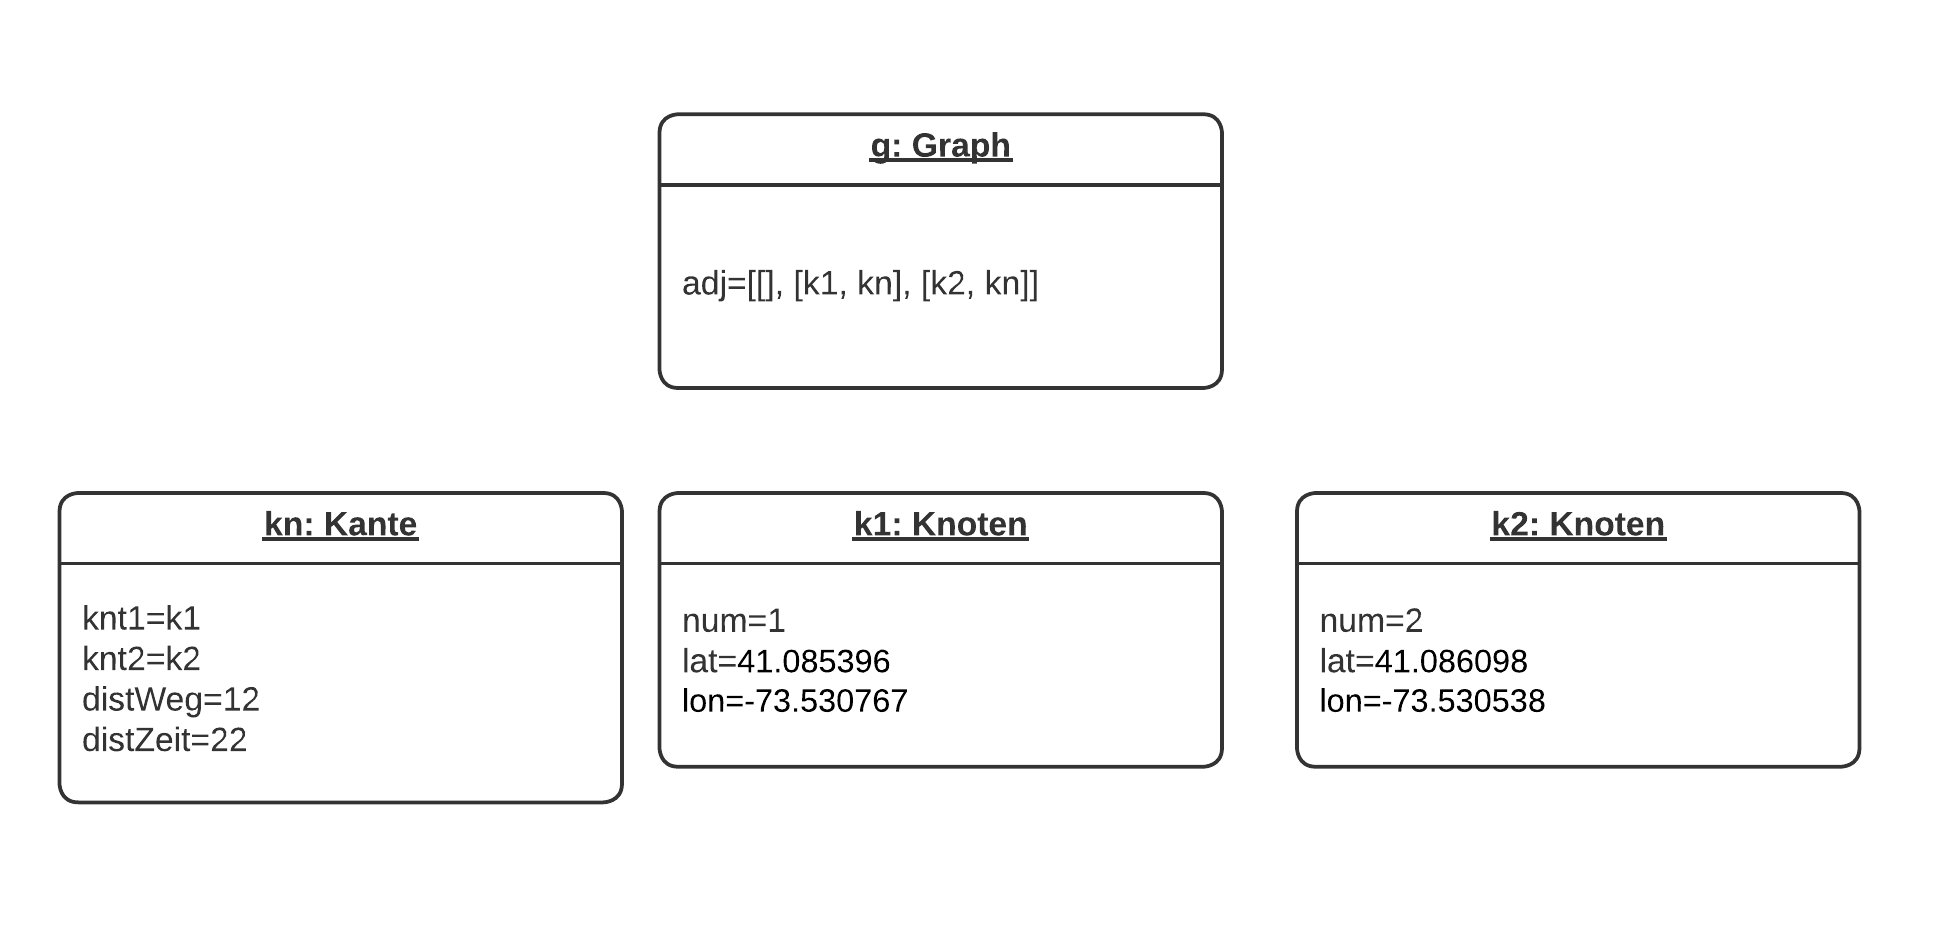
\includegraphics[width=\textwidth]{Objektdiagramm.png}
  \vspace{-1cm}
  \caption{Objektdiagramm}
\end{figure}

\begin{figure}[!ht]
  \center
  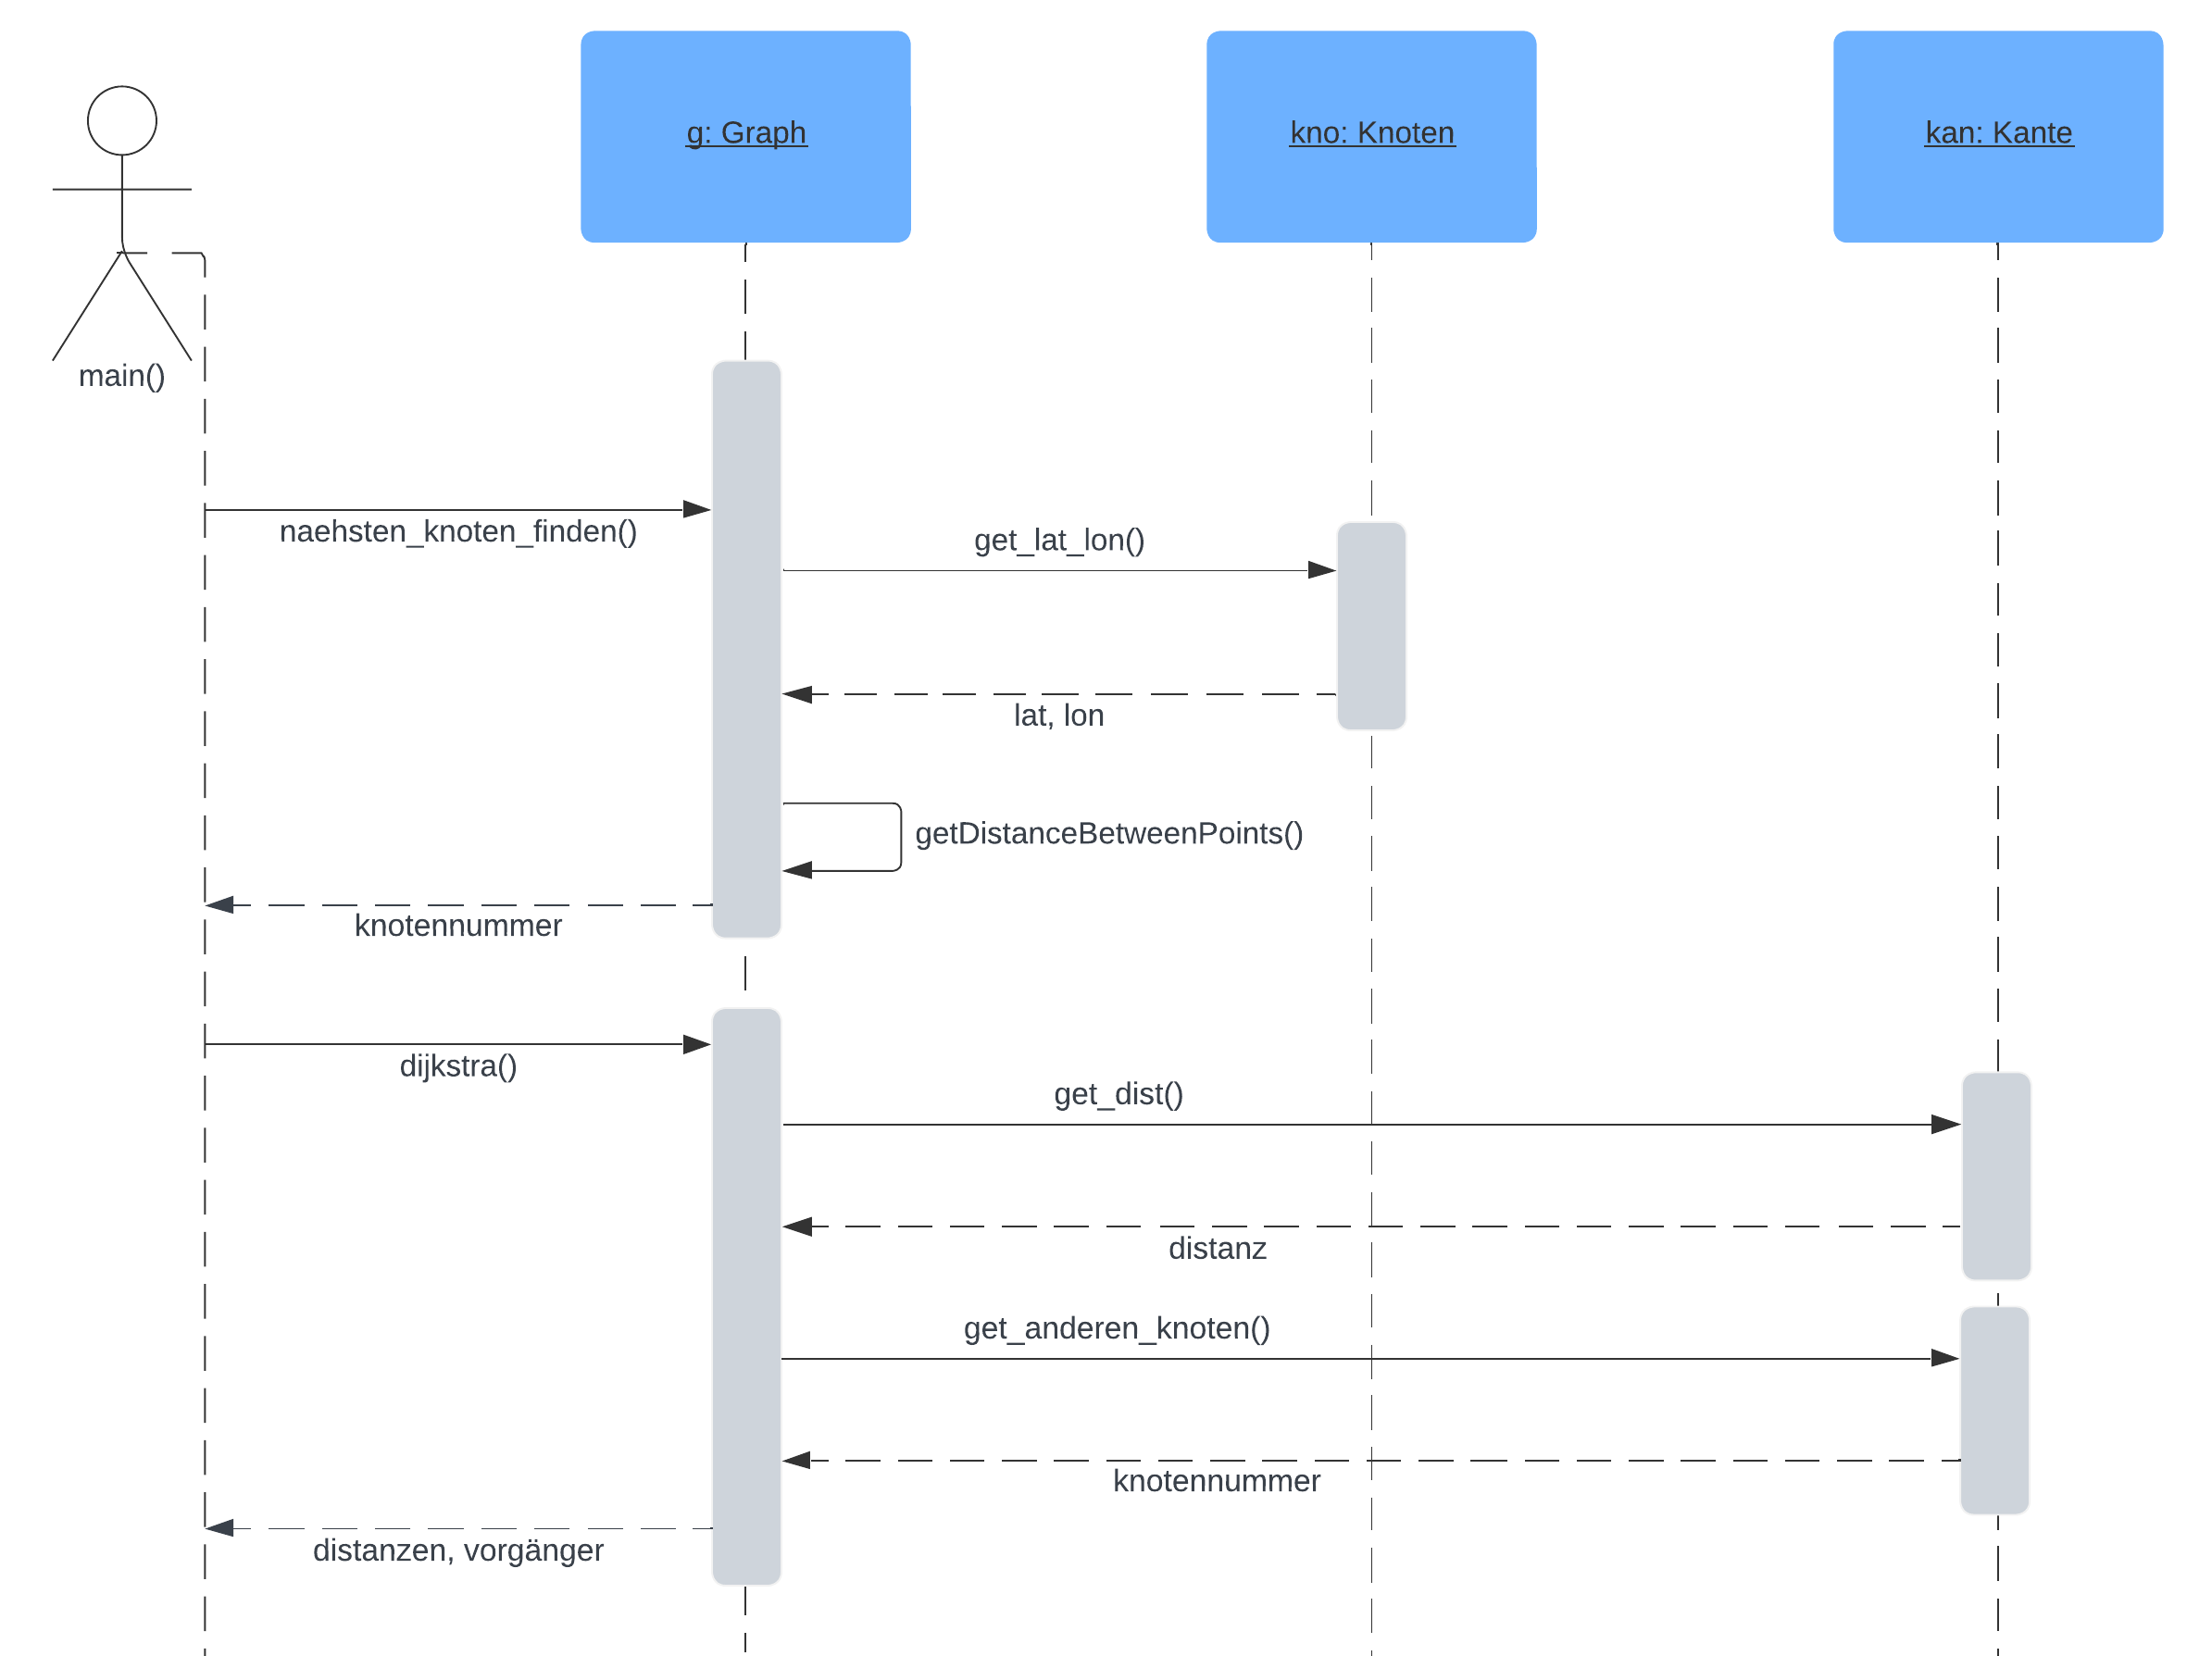
\includegraphics[width=\textwidth]{Sequenzdiagramm.png}
  \vspace{-.5cm}
  \caption{Sequenzdiagramm}
\end{figure}

\begin{figure}[!ht]
  \center
  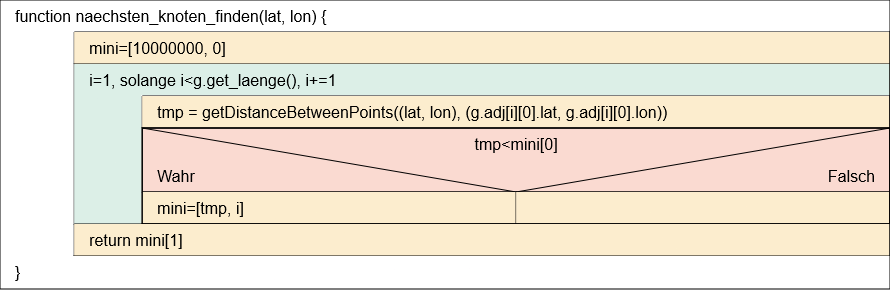
\includegraphics[width=\textwidth]{Struktogramm.png}
  \vspace{-1cm}
  \caption{Struktogramm für $naechsten\_knoten\_finden()$}
\end{figure}

\newpage
\section{Testungen und Vergleich mit Anforderungen}
Neben den von Python durchgeführten statischen Testverfahren wurden auch dynamische Testverfahren verwendet. Dazu wurden während der Implementierung Komponententests (ein Beispiel auskommentiert am Ende von backend.py) durchgeführt. Hier wurden die einzelnen Klassen und die einzelnen Funktionen mit Minimaltests, also einem Graphen mit nur zwei Knoten und einer Kante und mit den gegebenen Daten getestet, wobei dort sehr kurze Routen gewählt wurden, sodass sie nachvollziehbar waren. Auch im Frontend wurden die Komponenten, wie z.B. der Button, einzeln getestet. Das Zusammenspiel der Klassen und Funktionen wurde im Integrationstest getestet und das ganze System im Systemtest. Am Schluss fand der Auslieferungstest statt, bei dem die Webseite aus der Sicht des Kunden bedient wurde. Hier ergibt sich ein unbeachteter Extremfall, bei dem der Kunde so stark aus der Karte herauszoomen kann, dass die Weltkarte zweimal zu sehen ist und auch ein Punkt auf dem “zweiten New York” gewählt werden kann, wodurch die Route nicht berechnet werden kann. Dieses Problem ist allerdings auf das Paket folium zurückzuführen. \\
Damit konnten alle gestellten Anforderungen weitesgehend erfüllt werden. Allerdings ist auf der im Internet verfügbaren Webseite mit einer langen Laufzeit zu rechnen, da die dort genutzten Ressourcen nicht für die Datenmengen ausreichen. Wenn dies allerdings lokal betrieben wird, ist die Laufzeit akzeptabel. Auch ist aufgrund der ungenau angegebenen Koordinaten der Knoten des Straßennetzes in einigen Fällen eine minimale Verschiebung der Route von der Straße erkennbar.


\end{document}
